%-- Intro --%

\begin{tframe}{Introduction}

This method is based on \emph{T. Carvalho}, \emph{V. Schetinger et al. }works presented in [1] and [2].
\vspace{1cm}

\textbf{Main goal}: finding image inconsistencies based on \textbf{illuminant estimation} in order to determine if an image has been \textbf{tampered} or not.

\begin{center}
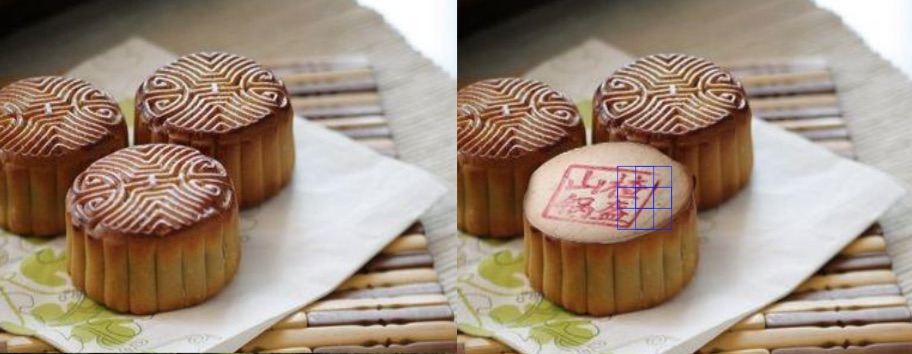
\includegraphics[width=0.6\textwidth]{images/cakes.jpg}
\end{center}

\end{tframe}

\begin{tframe}{Illuminant Maps estimation}
\vspace{0.2cm}
For the Illuminant Maps estimation, two different techniques are used: 
\vspace{0.3cm}
\begin{enumerate}
\item A \emph{statistical-based} approach using \textbf{Generalized Grayworld Estimate (GGE)} algorithm.
\vspace{0.2cm}
\item A \emph{physics-based} approach using \textbf{Inverse-Intensity Chromaticity (IIC)} method.
\end{enumerate}

\begin{center}
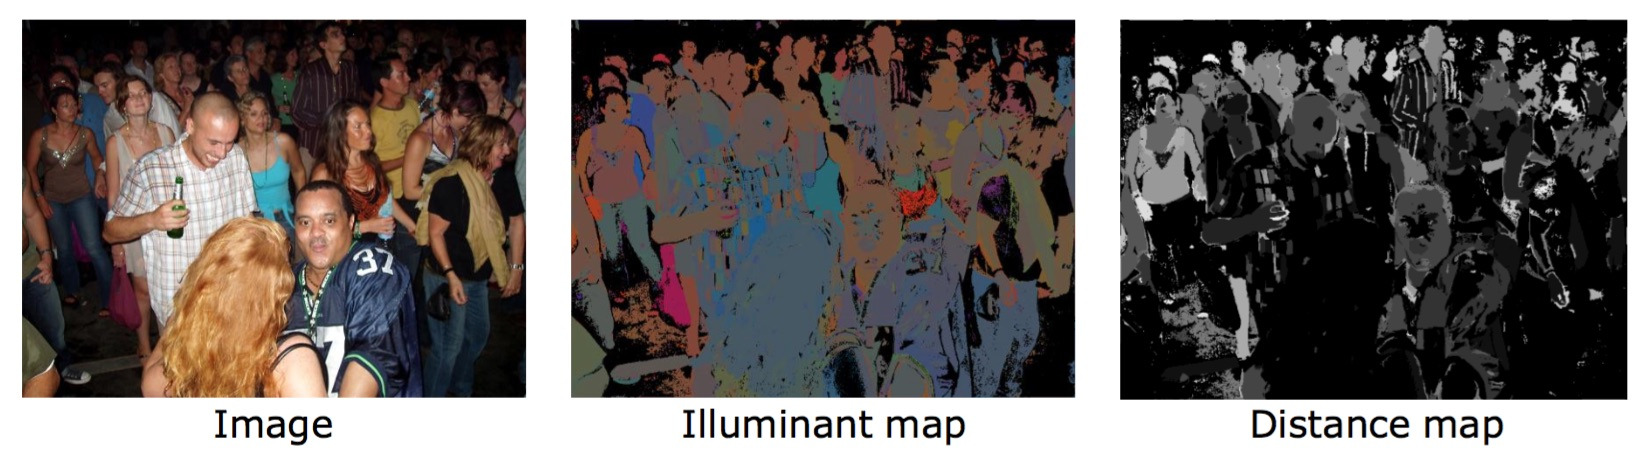
\includegraphics[width=0.7\textwidth]{images/riess.jpg}
\end{center}
\end{tframe}


\begin{tframe}{2.1 Generalized Greyworld Estimate (GGE)}
\textbf{Generalized Greyworld Estimate} is proposed in [2] as a combination of the \emph{Grey-World} and \emph{Grey-Edge method}s aimed to evaluate \textbf{color constancy}.

\vspace{0.3cm}
The main premise behind it is that in a normal well color balanced photo, the \textbf{average} of all the colors is a neutral gray. Therefore, it assumes that the \emph{Minkowski norm} of the derivative of the reflectance in a scene is \textbf{achromatic}.

\begin{equation}
k\textbf{e}^{n, p, \sigma} = (\int |\frac{\vartheta^{n}\textbf{f}^{\sigma}(\textbf{x})}{\vartheta\textbf{x}^{n}}|^{p}  d\textbf{x})^{\frac{1}{p}}
\end{equation}
\begin{footnotesize}
where $\textbf{x}$ denotes a pixel coordinate, $k$ is a scale factor, $|\cdot|$ is the absolute value operator, $\vartheta$ the partial differential operator, $\textbf{f}^{\sigma}$ is the observed intensities at position $\textbf{x}$, smoothed by a Gaussian kernel $\sigma$, $p$ is the \emph{Minkowski norm}, and $n$ is the derivative order.
\end{footnotesize}
\end{tframe}

\begin{tframe}{Generalized Greyworld Estimate (GGE)}

The illuminant estimation of (1) is a framework for low-level based illuminant estimation based on three variables:
\begin{enumerate}
\item The order $n$ of the image structure.
\item The Minkowski norm $p$ which determines the relative weights of the multiple measurements from which the final illuminant color is estimated.
\item The scale of the local measurements as denoted by $\sigma$.
\end{enumerate}
\vspace{0.2cm}
\textbf{Advantages}:
\begin{itemize}
\item the Minkowski norm of RGB values or derivatives can be computed\emph{ extremely fast}
\item the method does not require an image database taken under a \textbf{known light source}
\end{itemize}

\end{tframe}


\begin{tframe}{Inverse-Intensity Chromaticity (IIC)}
Extension of the \textbf{dichromatic reflectance model}, which states that \emph{the amount of light reflected from a point, $\textbf{x}$, of a dielectric, non-uniform material is a linear combination of diffuse reflection and specular reflection}.

\vspace{0.2cm}

Given an image taken with a \textbf{RGB camera}, the response $I_c(\textbf{x})$ for each color filter $c \in \{R, G, B\}$ is

$$
I_c(\textbf{x}) = m_d(\textbf{x})B_c(\textbf{x}) + m_s(\textbf{x})G_c(\textbf{x})
$$

\begin{small}
where $m_d$ and $m_s$ are geometric parameters of \textbf{diffuse and specular reflection}.
\vspace{0.2cm}

Let $\Delta_c(\textbf{x})$ and $\Gamma_c(\textbf{x})$ be the diffuse and \textbf{specular chromaticity}: $\Delta_c(\textbf{x}) = \frac{B_c(\textbf{x})}{\sum_{i in \{R, G, B\}} B_i(\textbf{x})}$ and $\Gamma_c(\textbf{x}) = \frac{G_c(\textbf{x})}{\sum_{i in \{R, G, B\}} G_i(\textbf{x})}$
\end{small}

\end{tframe}

\begin{tframe}{Inverse-Intensity Chromaticity (IIC)}

In this model, the intensity $I_c(\textbf{x})$ and the chromaticity $\sigma_c(\textbf{x})$ of a color channel $c \in \{R, G, B\}$ at pixel position $\textbf{x}$ are related by

\begin{equation}
\sigma_c(\textbf{x}) = p_c(\textbf{x}) \frac{1}{\sum_{i \in \{R, G, B\}} I_i(\textbf{x})} + \Gamma_c(\textbf{x})
\end{equation}
\vspace{0.2cm}

\begin{small}
where $p_c(\textbf{x}) = w_d(\textbf{x}) \sum_i B_i(\textbf{x}) (\Delta_c(\textbf{x}) - \Gamma_c(\textbf{x}))$ 
\end{small}

\begin{center}
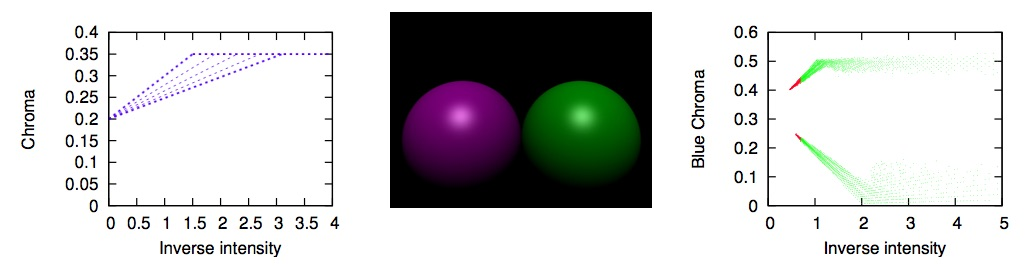
\includegraphics[width=0.6\textwidth]{images/iic.jpg}
\end{center}
The \emph{domain} of the line is determined by $\frac{1}{\sum_i I_i(\textbf{x})}$ and the \emph{range} is given by $0 \leq \sigma_c \leq 1$. Domain and range together form the \textbf{inverse-intensity chromaticity (IIC) space}.
\end{tframe}


